\documentclass[12pt,a4paper, reqno]{amsart}
\usepackage[slovene]{babel}
\usepackage[utf8]{inputenc}
%\usepackage[T1]{fontenc}
\usepackage{amsmath,amssymb,amsfonts}
\usepackage[dvipsnames,usenames]{color}
\usepackage{algorithmicx,algpseudocode}
\usepackage{graphicx}
\usepackage{wrapfig}
\usepackage{varwidth}
\usepackage{caption}
\captionsetup{justification   = centering,
              singlelinecheck = false}

\textwidth 15cm
\textheight 24cm
\oddsidemargin.5cm
\evensidemargin.5cm
\topmargin-5mm
\addtolength{\footskip}{10pt}
\pagestyle{plain}

\overfullrule=15pt % oznaci predlogo vrstico

\newtheorem{definicija}{Definicija}[section]
\newtheorem{lema}[definicija]{Lema}
\newtheorem{izrek}[definicija]{Izrek}
\newtheorem{trditev}[definicija]{Trditev}
\newtheorem{posledica}[definicija]{Posledica}

\let\oldref\ref
\renewcommand{\ref}[1]{(\oldref{#1})}

\def\R{\mathbb R}
\def\N{\mathbb N}
\def\Z{\mathbb Z}
\def\C{\mathbb C}
\def\Q{\mathbb Q}

\renewcommand{\algorithmicrequire}{{\bf Vhod:}}

\begin{document}

\thispagestyle{empty}
\noindent{\large
Univerza v Ljubljani \hfill Ljubljana, \today\\[1mm]
Fakulteta za matematiko in fiziko  \\[5mm]
%IŠRM -- 2.~stopnja 
}
\medskip
%\vfill
\begin{center}{\large
Računalniško podprto geometrijsko oblikovanje\\[4mm]
% Seminarska naloga\\[4mm]
{\bf Iskanje presečišč B\`{e}zierjevih krivulj z metodo hibridnih izrezkov}\\[4mm]
Domen Keglevič\\[6mm]
}
\end{center}
\medskip
% tu se zacne tekst seminarja
\section{Uvod}
V seminarski nalogi nas bo zanimalo kako najti presečišča dveh ravninskih B\`{e}zier\-jevih krivulj. Ta problem lahko opišemo na naslednji način. Naj bosta ${\bf f}:[\alpha,\beta]\rightarrow \R^2$ in ${\bf g}:[\xi,\eta]\rightarrow \R^2$ ravninski B\`{e}zierjevi krivulji. Želimo najti učinkovit algoritem, ki za poljuben $\epsilon >0$ vrne pare intervalov $[\alpha_i,\beta_i]$ in $[\xi_i,\eta_i]$, ki vsebujejo presečišča ${\bf f}(t_i) = {\bf g}(s_i)$, $t_i\in[\alpha_i,\beta_i]$, $s_i\in[\xi_i,\eta_i]$, tako da velja $|\alpha _i - \beta _i| < \epsilon$ in $|\xi _i - \eta _i| < \epsilon$.

Ta problem se da rešiti na več načinov. Tu bomo predstavili metodo hibridnih izrezkov, ki je razširitev metode B\`{e}zierjevih izrezkov. 

Metoda B\`{e}zierjevih izrezkov najprej aproksimira krivuljo ${\bf g}$ z ozkim pasom $\mathcal{L}$ v ravnini ({\em fat line}), tako da ${\bf g}$ leži znotraj $\mathcal{L}$. Nato izračuna presek pasa $\mathcal{L}$ in konveksne ovojnice kontrolnih točk krivulje ${\bf f}$, ter definicijsko območje krivulje ${\bf f}$ omeji na intervale, kjer je presek neprazen. 
Nato vlogi ${\bf f}$ in ${\bf g}$ zamenja in postopek ponavlja, dokler ne pride do željene natančnosti.

Ideja metode hibridnih izrezkov je podobna kot ideja metode B\`{e}zierjevih izrezkov, le da ne opazujemo presek pasa $\mathcal{L}$ s konveksno ovojnico kontrolnih točk krivulje ${\bf f}$, ampak z območjem $\mathcal{P}$ ({\em fat curve}). Tega dobimo tako, da z nižanjem stopnje krivulje ${\bf f}$ dobimo aproksimacijo, ki jo lahko premaknemo v dve nasprotni smeri tako, da je krivulja ${\bf f}$ vsebovana v območju $\mathcal{P}$ vmes (slika \ref{slika2}). Nato krivuljo ${\bf f}$ zmanjšamo na tiste intervale, kjer je presek $\mathcal{L}\cap\mathcal{P}$ neprazen. V naslednjem koraku vlogi ${\bf f}$ in ${\bf g}$ zamenjamo in postopek ponavljamo do željene natančnosti.
\begin{figure}[!h]
  \centering
    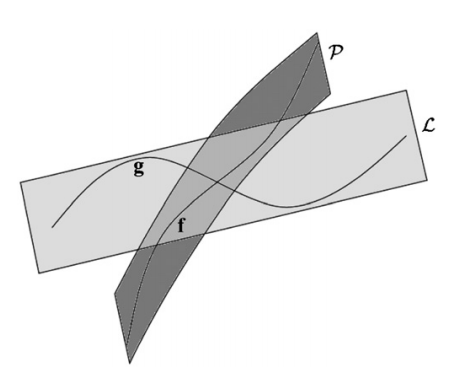
\includegraphics[width=0.45\linewidth]{2}
  	\caption{{\em Fat line $\mathcal{L}$} in {\em fat curve $\mathcal{P}$}, ki omejujeta {\bf g} in {\bf f}.}
  	\label{slika2}
\end{figure}
\medskip

\section{Metoda hibridnih izrezkov}
Vpeljimo nekaj oznak, ki jih bomo uporabljali v nadaljevanju. Z 
$$
B_{i,[\alpha,\beta]}^n(t) = \binom{n}{i} \frac{(t-\alpha)^i(\beta - t)^j}{(\beta - \alpha)^n}
$$
označimo $i$-ti Bernsteinov bazni polinom stopnje $n$ na intervalu $[\alpha,\beta]$. Intervale $[\alpha,\beta]$ namesto intervala $[0,1]$ opazujemo zato, ker bo algoritem generiral zaporedje vedno manjših intervalov.

Naj bosta ${\bf f}$ in ${\bf g}$ ravninski B\`{e}zierjevi krivulji dani z 
$${\bf f}(t) = \sum _{i=0}^{n} {\bf a}_i B_{i,[\alpha,\beta]}^n(t), \qquad t\in[\alpha,\beta]$$
in
$${\bf g}(s) = \sum _{j=0}^{m} {\bf b}_i B_{j,[\xi,\eta]}^m(s), \qquad s\in[\xi,\eta],$$
kjer so ${\bf a}_i, {\bf b}_j \in \R ^2$ kontrolne točke od ${\bf f}$ oz. ${\bf g}$. Naj bo $\lVert \,\cdot\,\rVert$ Evklidska norma na $\R^2$. Definiramo še naslednje norme:
\begin{enumerate}
\item Normalizirana $L_2$ norma
$$
\lVert {\bf f} \rVert _2^{[\alpha,\beta]} = \sqrt{\frac{1}{\beta -\alpha}\int _{\alpha}^{\beta}\lVert {\bf} f(t)\rVert ^2 dt},
$$
\item $L_{\infty}$ norma
$$
\lVert {\bf f} \rVert _\infty^{[\alpha,\beta]} = \max _{t\in[\alpha,\beta]} \lVert {\bf f}(t)\rVert,
$$
\item BB norma
$$
\lVert {\bf f} \rVert _{\text{BB}}^{[\alpha,\beta]} = \max _{i=0,\ldots,n} \lVert {\bf a}_i\rVert.
$$
\end{enumerate}


\subsection{{\em Fat line}}
Naj bo ${\bf n}$ normalni vektor, ki je pravokoten na ${\bf b}_m - {\bf b}_0$. Definiramo predznačeni razdalji 
\begin{gather*}
d_{\text{max}} = \max _{i=0,\ldots ,m} ({\bf n}\cdot ({\bf b}_i - {\bf b}_0)),\\
d_{\text{min}} = \min _{i=0,\ldots ,m} ({\bf n}\cdot ({\bf b}_i - {\bf b}_0)).
\end{gather*}
Množico $\mathcal{L}$, ki ga sestavljajo točke, ki so od premice ${\bf b}_0{\bf b}_m$ oddaljene kvečjemu za $d_{\text{min}}$ oz. $d_{\text{max}}$ imenujemo {\em fat line}. Krivulja ${\bf g}$ je vsebovana v $\mathcal{L}$, saj je v $\mathcal{L}$ vsebovana njena konveksna ovojnica.
\begin{figure}[!h]
    \centering 
    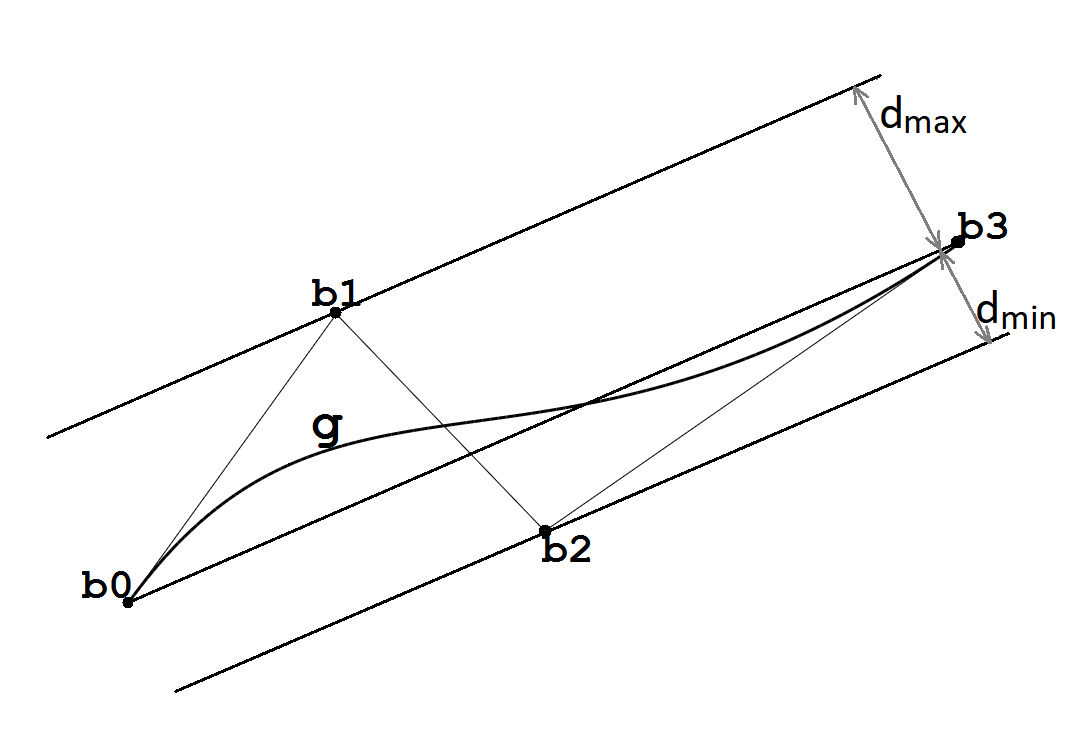
\includegraphics[width=0.5\textwidth]{fat_line}
    \caption{Krivulja {\bf g} in {\em fat line.}}
  	%\caption{{\em Fat line $\mathcal{L}$}.}
  	\label{slika3}
\end{figure}


\subsection{\em Fat curve}
Naj bo ${\bf \hat{p}}(t)$ polinom stopnje $k < n$, ki optimalno aproksimira ${\bf f}(t)$ glede na normo $L_2$. Konstruiramo ga s pomočjo nižanja stopnje krivulje ${\bf f}(t)$, kot je opisano v \textcolor{red}{referenca}. S pomočjo višanja stopnje mu lahko zvišamo stopnjo do $n$ in zapišemo
$$
{\bf \hat{p}}(t) = {\bf p}(t) = \sum _{i=0}^n {\bf c}_iB_{i,[\alpha,\beta]}^n(t),
$$
kjer so ${\bf c}_i$ nove kontrolne točke. Naj bo 
\begin{equation}\label{def_delta}
\delta = \lVert {\bf f}(t) - {\bf p}(t) \rVert _{BB}^{[\alpha,\beta]}.
\end{equation}
Velja naslednja ocena
$$
\lVert {\bf f}(t) - {\bf p}(t) \rVert = \lVert \sum _{i=0}^n({\bf a}_i-{\bf c}_i)B_{i,[\alpha,\beta]}^n(t) \rVert
\leq \sum _{i=0}^n\lVert{\bf a}_i-{\bf c}_i\rVert B_{i,[\alpha,\beta]}^n(t) \leq \delta.
$$
Sledi, da ${\bf f}(t)$ leži med ${\bf p}_1(t) = \hat{{\bf p}}(t) + \delta {\bf n}(t)$ in ${\bf p}_2(t) = \hat{{\bf p}}(t) - \delta {\bf n}(t)$, kjer je ${\bf n}$ normala pravokotna na ${\bf b}_m - {\bf b}_0$ (kot v {\em fat line}). Naj bo
\begin{gather*}
d(t) = {\bf n}\cdot({\bf f}(t) - {\bf b}_0), \, d_0(t)= {\bf n}\cdot ({\bf p}(t) - {\bf b}_0)\\
d_1(t) = {\bf n} ({\bf p}_1(t) - {\bf b}_0) = d_0(t) + \delta \\
d_2(t) = {\bf n} ({\bf p}_2(t) - {\bf b}_0) = d_0(t) - \delta.
\end{gather*}
Potem velja ocena
$$
|d(t)-d_0(t)|=|{\bf n}\cdot({\bf f}(t)-{\bf p}(t))|\leq \lVert {\bf n}\rVert\cdot \lVert {\bf f}(t) - {\bf p}(t) \rVert \leq \lVert {\bf f}(t) - {\bf p}(t) \rVert _{\infty}^{[\alpha,\beta]} \leq \delta.
$$
To pomeni, da $d(t)$ leži v pasu med $d_1(t)$ in $d_2(t)$ kot prikazuje slika \ref{slika4}.
\begin{figure}[!h]
    \centering 
    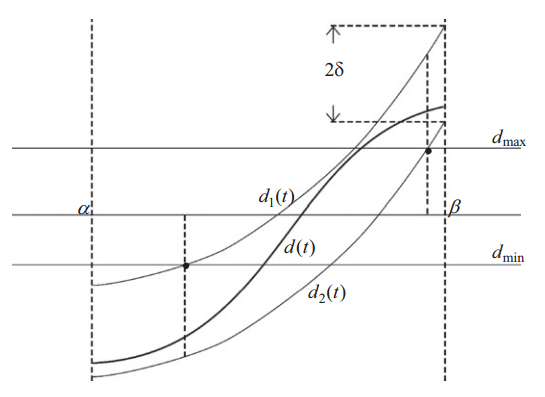
\includegraphics[width=0.6\textwidth]{dist}
    \caption{}
  	\label{slika4}
\end{figure}

\subsection{Iskanje intervalov}
Iz zgornjih dveh razdelkov vemo, da je (predznačena) razdalja točke ${\bf g}(t)$ od premice ${\bf b}_0{\bf b}_m$ med $d_{\text{min}}$ in $d_{\text{max}}$, ter da je (predznačena) razdalja točke ${\bf f}(t)$ od premice ${\bf b}_0{\bf b}_m$ med $d_1(t)$ in $d_2(t)$. Vsa tista območja, kjer je $d_1(t) < d_{\text{min}}$ in $d_2(t) > d_{\text{max}}$, lahko zavržemo. Natančneje, če najdemo rešitve enačb
$$
d_1(t) = d_{\text{min}} \, \text{ in } \, d_2(t) = d_{\text{max}},
$$
potem lahko v domeni krivulje ${\bf f}$ najdemo intervale $[\alpha _i, \beta _i]$, ki jih iščemo. V obeh enačbah iščemo ničle polinoma. Če smo krivuljo ${\bf f}$ aproksimirali s krivuljo stopnje $2$ ali $3$, potem lahko ti dve enačbi rešimo analitično, kar je v praksi najbolj učinkovita možnost.


\subsection{Psevdo koda algoritma}\text{}
\smallskip
\begin{small}
   \begin{algorithmic}[1]
	\Require $({\bf f},{\bf g}, [\alpha,\beta], [\xi,\eta], k)$ : ravninski B\`{e}zierjevi krivulji, njuni domeni in stopnja aproksimacijske krivulje

	\If{$|\alpha - \beta | < \epsilon$ in  $|\xi - \eta| < \epsilon$} \hfill ustavitveni pogoj
		\State \Return $[\alpha,\beta],[\xi,\eta]$
	\Else
		\If{$|\alpha - \beta | < |\xi - \eta|$} \hfill če ima {\bf f} manjšo domeno
			\State $HybridClip( {\bf g}, {\bf f}, [\xi,\eta],[\alpha,\beta],k)$ 
			\hfill zamenjamo vlogi ${\bf f}$ in ${\bf g}$
		\Else
			\State $L, C \gets $ {\em fat line}$({\bf g})$, {\em fat curve}$({\bf f})$ 
			\hfill aproksimiraj ${\bf f}$ in ${\bf g}$
			\State Najdi intervale $[\alpha _i,\beta _i]$, kjer je $L\cap C\neq \emptyset$
			\If{$l > 0$ in $\max _{i=1,\ldots ,l}\, \{ |\alpha _i - \beta _i|\} \geq 
				\frac{1}{2}|\alpha -\beta |$} \hfill  aproksimacija ni dobra
				\State \Return \begin{varwidth}[t]{\linewidth}  
					$HybridClip({\bf f},{\bf g},[\alpha,\frac{1}{2}(\alpha+\beta)],[\xi,\frac{1}{2}(\xi+\eta)],k)$\par $ 
        \hskip\algorithmicindent
					\cup \, HybridClip({\bf f},{\bf g},[\alpha,\frac{1}{2}(\alpha+\beta)],[\frac{1}{2}(\xi+\eta), \eta],k)$\par$
        \hskip\algorithmicindent
					\cup \, HybridClip({\bf f},{\bf g},[\frac{1}{2}(\alpha+\beta), \beta],[\frac{1}{2}(\xi+\eta), \eta],k)$\par$
        \hskip\algorithmicindent
					\cup \, HybridClip({\bf f},{\bf g},[\frac{1}{2}(\alpha+\beta), \beta],[\xi, \frac{1}{2}(\xi+\eta)],k)$
					\end{varwidth}
			\Else \hfill  aproksimacija je dobra
				\State $S\gets \emptyset$
				\For{$i=1,\ldots,l$} 
					\State $S\gets S\cup HybridClip({\bf f},{\bf g},[\alpha _i,\beta _i], [\xi,\eta],k)$
					\hfill rekurziven klic
				\EndFor
				\State \Return $S$ \hfill vrnemo rezultat
			\EndIf
		\EndIf
	\EndIf
   \end{algorithmic}
\end{small}
\smallskip

Klic funkcije $HybridClip({\bf f},{\bf g}, [\alpha,\beta],[\xi,\eta],k)$ vrne pare intervalov $[\alpha_i,\beta_i], [\xi_i,\eta_i]$, ki vsebujejo vsa presečišča in so manjši od predpisanega $\epsilon$. Lahko se zgodi, da med njimi vrne tudi par intervalov, kjer se krivulji ${\bf f }$ in ${\bf g}$ ne sekata, ampak le prideta blizu skupaj.


\subsection{Opombe}


\section{Red konvergence}

\begin{trditev}\label{norm_invariance}

\textcolor{red}{invarianca norm za afine transormacije}
\end{trditev}
\proof

\endproof

\begin{lema}\label{prvalema}
Naj bo ${\bf f}$ ravninska B\`{e}zierjeva krivulja in ${\bf p}$ njena optimalna $L_2$ aproksimacija stopnje $k$. Potem obstaja konstanta $C$, da za poljuben interval $[\alpha,\beta]\subseteq[0,1]$ velja $\lVert {\bf f} - {\bf p} \rVert _{BB}^{[\alpha,\beta]} \leq C |\alpha - \beta|^{k+1}$.
\end{lema}
\proof
Spomnimo se, da za poljubni normi $\lVert\, \cdot\, \rVert _1$ in $\lVert\, \cdot \,\rVert _2$ na končno dimenzionalnem vektorskem prostoru $V$ obstajata konstanti $0 < C_1 \leq C_2$, tako da je 
\begin{equation}\label{norm_equiv}
C_1 \lVert v\rVert _2 \leq \lVert v\rVert _1 \leq C_2 \lVert v\rVert _2, \; v\in V.
\end{equation}
Zato obstajata konstanti $D_1$ in $D_2$, da je $\lVert {\bf r}\rVert _{BB}^{[\alpha,\beta]} \leq D_1 \lVert {\bf r}\rVert _2^{[\alpha,\beta]}$ in $\lVert {\bf r}\rVert _{2}^{[\alpha,\beta]} \leq D_2 \lVert {\bf r}\rVert _\infty^{[\alpha,\beta]}$ za vsak ${\bf r}\in  \Pi _{[\alpha,\beta]}^n$. Pri tem konstanti $D_1$ in $D_2$ nista odvisni od intervala $[\alpha,\beta]$, saj so po trditvi \ref{norm_invariance} norme invariantne glede na afine transformacije.

Od tod sledi, da je 
$\lVert {\bf f} - {\bf p} \rVert _{BB}^{[\alpha,\beta]} \leq D_1 \lVert {\bf f} - {\bf p} \rVert _{2}^{[\alpha,\beta]}$. Naj bodo komponente ${\bf q}_\alpha$ Taylorjevi polinomi stopnje $k$ razviti okrog točke $t = \alpha$ za vsako komponento krivulje ${\bf f}$. Potem velja
$$
D_1 \lVert {\bf f} - {\bf p} \rVert _{2}^{[\alpha,\beta]} \leq D_1 \lVert {\bf f} - {\bf q}_\alpha \rVert _{2}^{[\alpha,\beta]},
$$
saj je ${\bf p}$ optimalna $L_2$ aproksimacija za ${\bf f}$. Iz \ref{norm_equiv} sledi, da je 
$
D_1 \lVert {\bf f} - {\bf q}_\alpha \rVert _{2}^{[\alpha,\beta]} \leq D_1D_2 \lVert {\bf f} - {\bf q}_\alpha \rVert _{\infty}^{[\alpha,\beta]}
$. Spomnimo se, da lahko razliko med ${\bf f}(t) - {\bf q}_\alpha(t)$ zapišemo v obliki
$$
{\bf f}(t) - {\bf q}_\alpha(t) = \frac{{\bf f}^{(k+1)}(t_o)}{(k+1)!}(t-\alpha)^{k+1},
$$
kjer je ${\bf f}^{(k+1)}$ $(k+1)$-vi odvod krivulje ${\bf f}$ in kjer vse člene opazujemo po komponentah. Od tod dobimo oceno
$$
D_1D_2 \lVert {\bf f} - {\bf q}_\alpha \rVert _{\infty}^{[\alpha,\beta]} \leq
\frac{\sqrt{2}}{(k+1)!}D_1D_2\max _{t\in [0,1]} \lVert {\bf f}^{(k+1)}(t_0) \rVert |\alpha - \beta|^{k+1}.
$$
\endproof

\begin{lema}\label{drugalema}
Naj bo ${\bf f}$ ravninska B\`{e}zierjeva krivulja stopnje $n$. Potem obstajajo konstante $C_{j}$, tako da za poljuben interval $[\alpha,\beta]\subseteq[0,1]$ in optimalno $L_2$ aproksimacijo ${\bf p}$ stopnje $k$ od ${\bf f}$ velja
$\lVert {\bf f}^{(j)} - {\bf p}^{(j)} \rVert _{\infty} \leq C_{j}|\alpha - \beta|^{k+1-j}$, za $j=0,1,\ldots,k$. 
\end{lema}
\proof
Definirajmo novo normo z naslednjim predpisom
$$
\lVert {\bf r}\rVert _{*}^{[\alpha,\beta]} = \lVert {\bf r}\rVert _\infty^{[\alpha,\beta]} + |\alpha - \beta|\lVert {\bf r}'\rVert _\infty^{[\alpha,\beta]} + \ldots + 
 |\alpha - \beta|^k\lVert {\bf r}^{(k)}\rVert _\infty^{[\alpha,\beta]}.
$$
To je res norma, saj je $\lVert \,\cdot\, \rVert _\infty$ norma. Po trditvi \ref{norm_invariance} in iz \textcolor{Red}{neka referenca} sledi, da obstaja konstanta $D_1$, da je 
$$
\lVert {\bf r}\rVert _{*}^{[\alpha,\beta]} \leq D_1 \lVert {\bf r}\rVert _{2}^{[\alpha,\beta]}.
$$
S pomočjo te ocene lahko zapišemo 
\begin{align*}
\lVert {\bf f} - {\bf p}\rVert _{*}^{[\alpha,\beta]}  =  \lVert {\bf f} - {\bf p}\rVert _\infty^{[\alpha,\beta]}  &+  |\alpha - \beta|\lVert {\bf f}' - {\bf p}'\rVert _\infty^{[\alpha,\beta]} + \ldots +\\ 
   & +  |\alpha - \beta|^k\lVert {\bf f}^{(k)} - {\bf p}^{(k)}\rVert _\infty^{[\alpha,\beta]} \leq 
 D_1 \lVert {\bf f} - {\bf p}\rVert _{2}^{[\alpha,\beta]}
\end{align*}
Sedaj podobno kot v lemi \ref{prvalema} s pomočjo Taylorjevega polinoma in izreka o ostanku ocenimo
\begin{align*}
D_1 \lVert {\bf f} - {\bf p}\rVert _{2}^{[\alpha,\beta]} \leq 
D_1 \lVert {\bf f} - {\bf q}_\alpha\rVert _{2}^{[\alpha,\beta]} \leq 
D_1D_2 \lVert {\bf f} - &{\bf q}_\alpha\rVert _{\infty}^{[\alpha,\beta]} \leq \\
\frac{\sqrt{2}}{(k+1)!}  D_1D_2\max _{t\in [0,1]}& \lVert {\bf f}^{(k+1)}(t_0) \rVert |\alpha - \beta|^{k+1}.
\end{align*}
\endproof

\begin{definicija}
%\in
%\in \Pi _{[\xi,\eta]}^m
Naj bosta ${\bf f}(t)$ in ${\bf g}(s)$ ravninski B\`{e}zierjevi krivulji s presečiščem ${\bf z}_0 = {\bf f}(t_0) = {\bf g}(s_0)$. Presečišče ${\bf z}_0$ imenujemo:
\begin{itemize}
	\setlength\itemsep{0.33em}
\item {\em transverzalno presečišče}, če je ${\bf f}'(t_0)\times {\bf g}'(s_0) \neq {\bf 0}$,
\smallskip
\item {\em tangentno presečišče}, če je ${\bf f}'(t_0)\times {\bf g}'(s_0) = {\bf 0}$ in ${\bf f}'(t_0)\neq {\bf 0}$, ${\bf g}'(s_0)\neq {\bf 0}$, 
\smallskip
\item {\em degenerirano presečišče}, če je ${\bf f}'(t_0) = {\bf 0}$ ali ${\bf g}'(s_0) = {\bf 0}$.
\end{itemize}
\end{definicija}


\begin{trditev}
Naj imata Bezierjevi krivulji ${\bf f}$ in ${\bf g}$ transverzalno presečišče v ${\bf f}(t_0)={\bf g}(s_0)$. Potem obstajajo konstante $C_f, C_f', C_g$ in $C_g'$, da za dovolj velike $i\in \N$ velja
\begin{equation}\label{prva_neenakost}
|\alpha _{i+1} - \beta _{i+1}| \leq C_f |\alpha _{i} - \beta _{i}|^{k+1} + C_g|\xi _{i} - \eta _{i}|^2
\end{equation}
oz.
\begin{equation}\label{druga_neenakost}
|\xi _{i+1} - \eta _{i+1}| \leq C_f' |\alpha _{i} - \beta _{i}|^{2} + C_g'|\xi _{i} - \eta _{i}|^{k+1}.
\end{equation}
\end{trditev}

\proof
Dokazali bomo le neenakost \ref{prva_neenakost}, saj je dokaz za \ref{druga_neenakost} podoben. 

Naj bosta $[\alpha _i,\beta _i]$ in $[\xi _i,\eta _i]$ zaporedji intervalov, ki jih algoritem generira. Oglejmo si kako se algoritem obnaša za velike $i$. Ker se dolžine intervalov v vsakem koraku zmanjšajo vsaj za polovico, je 
\begin{equation*}
\lim _{i\rightarrow \infty} |\alpha _i-\beta _i| = 0 \,\text{ in }\, \lim _{i\rightarrow \infty} |\xi _i - \eta _i| = 0.
\end{equation*}
 Sledi, da ${\bf b}_0{\bf b}_m$ konvergira proti tangenti ${\bf g}'(s_0)$. Zato gre normala ${\bf n}$ na ${\bf b}_0{\bf b}_m$ proti normali ${\bf n}_0$ na ${\bf g}(s_0)$.

Naj bo $\omega = {\bf n}_0\cdot {\bf f}'(t_0)$. Po predpostavki je ${\bf f}'(t_0)\times {\bf g}'(s_0) \neq {\bf 0}$, torej je $\omega \neq 0$.

Oglejmo si situacijo v $i$-tem koraku algoritma, ki jo prikazuje slika \ref{slika1}. Velja 
$$
|\alpha _{i+1}-\beta _{i+1}| = h_{i+1,{\bf f}} \leq L_{i+1} = l_{i+1,1} + l_{i+1,2} + l_{i+1,3}.
$$
Želimo oceniti člene na desni strani neenakosti. Ker je $\frac{\omega}{4} = \frac{d_{max}-d_{min}}{l_{i+1,1}  + l_{i+1,3}}$ je
\begin{equation}
l_{i+1,1}  + l_{i+1,3} = \frac{4(d_{max} - d_{min})}{\omega}.
\end{equation}
Želimo oceniti še člen $l_{i+1,2}$. V ta namen si najprej oglejmo ali sta funkciji $d_1(t)$ in $d_2(t)$ naraščajoči. Najprej opazimo, da obstaja tak $\epsilon _1>0$, da je za dovolj velike $i$  
\begin{equation}\label{prva_ocena}
|d'(t_0) - \omega| = |{\bf n}\cdot {\bf f}'(t_0) - {\bf n}_0 \cdot {\bf f}'(t_0)| < \frac{\omega}{4},
\end{equation}
ko je $|\xi _i - \eta _i| < \epsilon _1$, saj gre ${\bf n}$ proti ${\bf n}_0$, ko $i\rightarrow\infty$. Obstaja tudi tak $\epsilon _2 > 0$, da je za dovolj velike $i$
\begin{equation}\label{druga_ocena}
\lVert {\bf f}'(t) - {\bf f}'(t_0)\rVert < \frac{\omega}{4},
\end{equation}
ko je $|\alpha _i - \beta _i| < \epsilon _2$ saj je ${\bf f}'$ zvezna. Dalje obstaja tudi tak $\epsilon _3 > 0$, da za dovolj velike $i$ velja
\begin{equation}\label{tretja_ocena}
|d'(t)-d'_1(t)| < \frac{\omega}{4},
\end{equation}
ko je $|\alpha _i - \beta _i| < \epsilon _3$, saj po lemi \ref{drugalema} velja
$$
|d'(t)-d'_1(t)| = |{\bf n}\cdot ({\bf f}'(t) - {\bf p}'(t))| \leq \lVert {\bf f}'(t) - {\bf p}'(t) \rVert \leq \lVert {\bf f}'(t) - {\bf p}'(t) \rVert _{\infty}^{[\alpha,\beta]} \leq C|\alpha _i- \beta_i|^k.
$$
Naj bo $\epsilon _4 = \min (\epsilon _1, \epsilon _2, \epsilon _3)$. S pomočjo ocen \ref{prva_ocena} in \ref{druga_ocena} lahko ocenimo
\begin{equation*}
\begin{split}
|d'(t)-\omega| & = |{\bf n}\cdot {\bf f}'(t) - {\bf n}_0\cdot{\bf f}'(t_0)| \\
& \leq |{\bf n}\cdot {\bf f}'(t) - {\bf n}\cdot{\bf f}'(t_0)| + 
|{\bf n}\cdot {\bf f}'(t_0) - {\bf n}_0\cdot{\bf f}'(t_0)|\\
&\leq \lVert {\bf f}'(t) - {\bf f}'(t_0)\rVert + |d'(t_0)-\omega|\\
&\leq \frac{\omega}{4} + \frac{\omega}{4} = \frac{\omega}{2},
\end{split}
\end{equation*}
za vse dovolj velike $i$, tako da je $|\alpha _i-\beta _i| < \epsilon _4$ in $|\xi _i - \eta _i| < \epsilon _4$. Zato je 
\begin{equation}\label{ocena_omega}
d'(t)<\frac{\omega}{2},
\end{equation}
 in skupaj z \ref{tretja_ocena} dobimo, da je $d_1'(t) = d_2'(t) > \frac{\omega}{4}$. Torej smo ugotovili, da sta funkciji $d_1(t)$ in $d_2(t)$ strogo naraščajoči na dovolj poznih intervalih $[\alpha _i, \beta _i]$.

Od tod sledi, da za poljuben $y_0$, za katerega velja $d_1(\alpha _i) < y_0 < d_2(\beta _i)$, velja, da imata enačbi $d_1(t)=y_0$ in $d_2(t) = y_0$ rešitvi $t_1$ in $t_2$ na intervalu $[\alpha _i, \beta _i]$. Zato je
$$
l_{i+1, 2} \leq \sup _{y_0\in (d_1(\alpha _i), d_2(\beta _i))} \{ |t_1-t_2|\, ; \, d_1(t_1)=d_2(t_2)=y_0\}.
$$
Če najdemo oceno za $|t_1-t_2|$, potem lahko s pomočjo zgornje enačbe ocenimo $l_{i+1,2}$. Oceno za $|t_1-t_2|$ bomo dobili na sledeč način. 
Opazimo, da za $d_1(t_1) = d_2(t_2) = y_0$ velja
$$
{\bf n}\cdot ({\bf p} (t_1) - {\bf p}(t_2)) = 2\delta,
$$
kjer je $\delta$ kot v \ref{def_delta}. Naj bo ${\bf p}(t)=(x(t),y(t))$. Potem po Lagrange-ovem izreku o srednji vrednosti obstajata takšna $t^{\star}$ in $t^{\diamond}$, da je
$$
{\bf p}(t_1) - {\bf p}(t_2) = (x(t_1) - x(t_2), y(t_1) - y(t_2)) = (x'(t^{\star})(t_1-t_2),y'(t^{\diamond})(t_1-t_2)).
$$
Od tod dobimo oceno
\begin{equation*}
\begin{split}
|{\bf n}\cdot(x'(t^{\star}), &y'(t^\diamond)) - d'(t)|  \\
& = |{\bf n} (x'(t^\star), y'(t^\diamond)) - {\bf n}\cdot {\bf f}'(t) | \\
& \leq \lVert (x'(t^\star), y'(t^\diamond)) - {\bf f}'(t)\rVert \\
& = \lVert (x'(t^\star),y'(t^\star)) - {\bf f}'(t) + (0, y'(t^\diamond)) - (0,y'(t^\star))\rVert \\
& \leq \lVert {\bf p}'(t^\star) - {\bf f}'(t)\rVert + \lVert {\bf p}'(t^\diamond) - {\bf p}'(t^\star)\rVert \\ 
& \leq \lVert {\bf p}'(t^\star) - {\bf p}'(t)\rVert + \lVert {\bf p}'(t) - {\bf f}'(t)\rVert + 
\lVert {\bf p}'(t^\diamond) - {\bf p}'(t^\star)\rVert \\
& \leq 2\max _{t^1,t^2\in [\alpha _i,\beta _i]} \lVert {\bf p}'(t^1) - {\bf p}'(t^2)\rVert + 
\lVert {\bf p}'(t) - {\bf f}'(t)\rVert _{\infty}^{[\alpha _i,\beta _i]}.
\end{split}
\end{equation*}
Po lemi \ref{drugalema} in ker je ${\bf p'}(t)$ enakomerno zvezna na $[\alpha _i,\beta _i]$ obstaja $\epsilon _5 > 0$, da za dovolj velike $i$ velja 
\begin{gather*}
\max _{t^1,t^2\in [\alpha _i,\beta _i]} \lVert {\bf p}'(t^1) - {\bf p}'(t^2)\rVert < \frac{\omega}{16},\\
\lVert {\bf p}'(t) - {\bf f}'(t)\rVert _{\infty}^{[\alpha _i,\beta _i]} < \frac{\omega}{8},
\end{gather*}
ko je $|\alpha _i - \beta _i| < \epsilon _5$. Naj bo $\epsilon _0 = \min (\epsilon _4, \epsilon _5)$. Potem je 
$$
|{\bf n}\cdot (x'(t^\star), y'(t^\diamond)) - d'(t)| < \frac{\omega}{4},
$$
ko je $|\alpha _i - \beta _i| < \epsilon _0$ in $|\xi _i - \eta _i| < \epsilon _0$.
Če \ref{ocena_omega} kombiniramo z zgornjo neenakostjo dobimo oceno
$$
{\bf n}\cdot (x'(t^\star), y'(t^\diamond)) > \frac{\omega}{4}.
$$
Ker je $2\delta _i = {\bf n}\cdot({\bf p}(t_1) - {\bf p}(t_2)) = (t_1-t_2){\bf n}\cdot(x'(t^\star),y'(t^\diamond))$, dobimo
$$
|t_1-t_2| < \frac{2\delta _i}{\omega /4 } = \frac{8\delta _i}{\omega}.
$$


\endproof
\begin{figure}[!h]
%\begin{figure}
  \begin{center}
    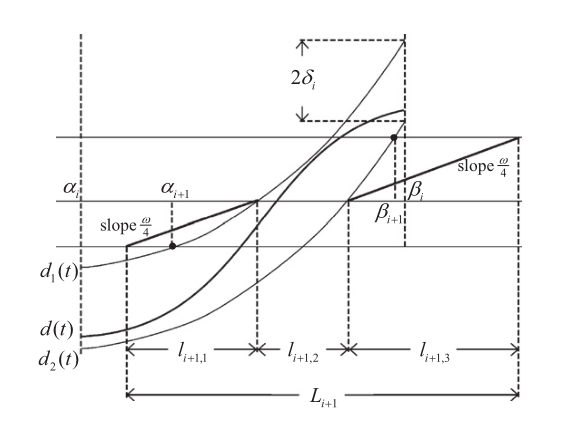
\includegraphics[width=0.7\linewidth]{1}
  \caption{Situacija v $i$-tem koraku algoritma.}
  \label{slika1}
  \end{center}
%  \end{figure}

\end{figure}

\section{Zaključki}
grafi, komentarji
% seznam uporabljene literature
\begin{thebibliography}{99}

\bibitem{bez_clip}
 Sederberg T, Nishita T. Curve intersection using B\`{e}zier clipping. Comput
Aided Des 1990;22(9):538--49.

\bibitem{oznaka-enote-za-sklic}
\textcolor{Red}{I.~Priimek, {\em Naslov "clanka}, okraj"sano ime revije {\bf letnik revije} (leto izida) strani od--do.}

\bibitem{navodilaOMF}
\textcolor{Red}{C.~Velkovrh, {\em Nekaj navodil avtorjem za pripravo rokopisa}, Obzornik mat.\ fiz.\ {\bf 21} (1974) 62--64.}

\end{thebibliography}

\end{document}

